\documentclass[12pt]{article}
\usepackage{amsmath, amssymb, amsthm}
\usepackage{geometry}
\usepackage{mathtools}
\geometry{margin=1in}
\usepackage{tikz}
\usetikzlibrary{arrows.meta, calc, decorations.markings}

\title{Lecture Notes: Differential 1-Forms and Scalar Projections on Curves}
\author{Mathematical Structures of Differential Forms}
\date{}

\begin{document}
	\maketitle
	
	\section*{1. A 1-Form on \(\mathbb{R}^2\) as a Scalar Projection}
	
	Let \( C \subseteq \mathbb{R}^2 \) be a smooth curve defined locally as the graph of a function \( f: \mathbb{R} \to \mathbb{R} \), i.e.,
	\[
	C = \{ (x, f(x)) \mid x \in \mathbb{R} \}.
	\]
	
	Let \( p = (a, f(a)) \in C \) be a fixed point on the curve. The derivative of \( f \) at \( a \), denoted \( f'(a) \), determines the tangent vector
	\[
	\vec{v} = \left\langle 1, f'(a) \right\rangle \in T_p C.
	\]
	
	Thus, the tangent space to the curve at point \( p \), denoted \( T_p C \), is
	\[
	T_p C = \text{span} \left\{ \left\langle 1, f'(a) \right\rangle \right\}.
	\]
	
	We aim to describe a differential 1-form on \( \mathbb{R}^2 \) that projects tangent vectors at \( p \) onto the line in direction \( \vec{v} \), i.e., the scalar projection.
	
	\subsection*{2. Geometric Identification}
	
	\textbf{Point vs. Tangent Vector Distinction:}
	
	- A point \( p \in C \subseteq \mathbb{R}^2 \) is a geometric location in space.
	- A vector \( \vec{w} \in T_p C \subseteq \mathbb{R}^2 \) is an element of the tangent space at \( p \); it encodes a direction and magnitude but is anchored at the point \( p \).
	
	\subsection*{3. Coordinate Systems}
	
	Define a coordinate system on \( C \) locally near \( p \) via the chart:
	\[
	(x,y): C \to \mathbb{R}^2,\quad q \mapsto (x(q), y(q)) = (x, f(x)).
	\]
	
	On the tangent space \( T_p C \), the natural dual basis of the cotangent space is given by the differentials:
	\[
	\langle dx, dy \rangle: T_p C \to \mathbb{R},\quad \vec{w} \mapsto \left( dx(\vec{w}), dy(\vec{w}) \right).
	\]
	
	More abstractly:
	\[
	x, y : C \to \mathbb{R}, \quad dx, dy: T_p C \to \mathbb{R}.
	\]
	
	\subsection*{4. Scalar Projection as a 1-Form}
	
	Define a unit vector in the direction of \( \vec{v} \):
	\[
	\hat{v} = \frac{1}{\sqrt{1 + (f'(a))^2}} \left\langle 1, f'(a) \right\rangle.
	\]
	
	The differential 1-form \( \omega \in \Omega^1(\mathbb{R}^2) \) which projects vectors onto \( \vec{v} \) is defined by:
	\[
	\omega = \frac{1}{\sqrt{1 + (f'(a))^2}} \left( dx + f'(a) \, dy \right).
	\]
	
	Then for any vector \( \vec{w} \in T_p C \), the evaluation \( \omega(\vec{w}) \) gives the scalar projection of \( \vec{w} \) onto the direction of \( \vec{v} \).
	
	\subsection*{5. Summary}
	
	- The 1-form \( \omega \) captures the infinitesimal scalar projection onto the tangent line of the curve.
	- The construction uses the differential of coordinate functions and normalization by the Euclidean norm.
	- This provides a clear geometric interpretation of a 1-form as a linear functional evaluating directional components of tangent vectors.
	
	\newpage
	\section*{Geometric Setting and 1-Form Construction}
	
	Let \( C \subseteq \mathbb{R}^2 \) be a curve given locally by the graph of a smooth function \( f(x) \), with
	\[
	C = \{ (x, f(x)) \mid x \in \mathbb{R} \}.
	\]
	Let \( p = (a, f(a)) \in C \), and let \( f'(a) \) be the derivative at \( x = a \). Then the tangent vector at \( p \) is
	\[
	\vec{v} = \left\langle 1, f'(a) \right\rangle.
	\]
	The tangent space is
	\[
	T_pC = \text{span}\left\{ \left\langle 1, f'(a) \right\rangle \right\}.
	\]
	
	We define a 1-form \( \omega \in \Omega^1(\mathbb{R}^2) \) by
	\[
	\omega = \frac{1}{\sqrt{1 + (f'(a))^2}} \left( dx + f'(a) \, dy \right),
	\]
	so that for any \( \vec{w} \in T_p \mathbb{R}^2 \), \( \omega(\vec{w}) \) gives the scalar projection onto the line in direction \( \vec{v} \).
	
	\section*{TikZ Visualization}
	
	\begin{center}
		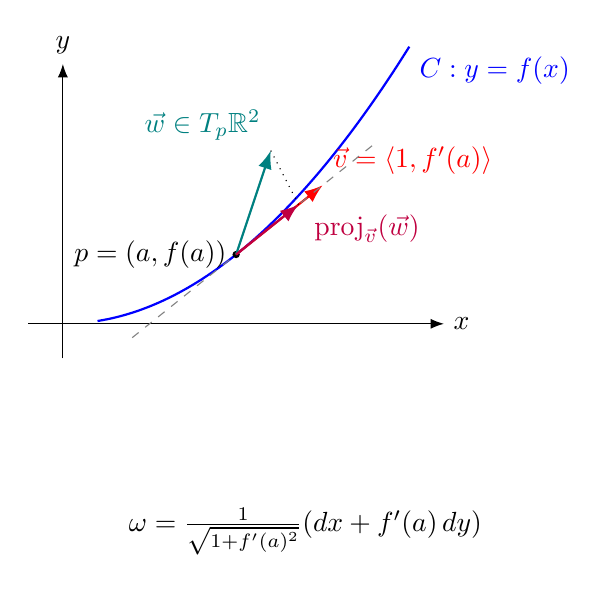
\begin{tikzpicture}[scale=2.2, >=Latex]
			
			% Axes
			\draw[->] (-0.2,0) -- (2.2,0) node[right] {\(x\)};
			\draw[->] (0,-0.2) -- (0,1.5) node[above] {\(y\)};
			
			% Curve f(x) = 0.4x^2
			\draw[domain=0.2:2, smooth, thick, blue] plot(\x,{0.4*\x*\x}) node[below right] {\(C: y = f(x)\)};
			
			% Point p = (1, f(1))
			\coordinate (P) at (1, 0.4);
			\filldraw[black] (P) circle (0.5pt) node[left] {\(p=(a,f(a))\)};
			
			% Tangent vector at p: <1, f'(a)> = <1, 2*0.4*1> = <1,0.8>
			\coordinate (T) at ($(P)+(0.5,0.4)$);
			\draw[->, thick, red] (P) -- (T) node[above right] {\(\vec{v} = \langle 1, f'(a) \rangle\)};
			
			% Dashed tangent line
			\draw[dashed, gray] ($(P)+(-0.6,-0.48)$) -- ($(P)+(0.8,0.64)$);
			
			% Another vector w at p
			\coordinate (W) at ($(P)+(0.2,0.6)$);
			\draw[->, thick, teal] (P) -- (W) node[above left] {\(\vec{w} \in T_p\mathbb{R}^2\)};
			
			% Projection of w onto v
			\coordinate (Proj) at ($(P)+(0.36,0.288)$);
			\draw[dotted] (W) -- (Proj);
			\draw[->, thick, purple] (P) -- (Proj) node[below right, xshift=2pt] {\(\text{proj}_{\vec{v}}(\vec{w})\)};
			
			% Label for 1-form omega
			\node at (1.4,-1.2) {\(\omega = \frac{1}{\sqrt{1 + f'(a)^2}}(dx + f'(a)\,dy)\)};
			
		\end{tikzpicture}
	\end{center}
	
	\section*{Interpretation}
	\begin{itemize}
		\item The red vector \( \vec{v} \) is the tangent to the curve \( C \) at point \( p \).
		\item The vector \( \vec{w} \in T_p\mathbb{R}^2 \) is arbitrary.
		\item The 1-form \( \omega \) computes the scalar projection of \( \vec{w} \) onto the direction of \( \vec{v} \).
		\item The 1-form has constant coefficients along the direction of \( \vec{v} \), normalized to unit length.
	\end{itemize}
	
	
\end{document}
